\chapter{Analisi a n-dimensioni}
\section{Tipo di testing}

Il testing eseguito si basa interamente sul software Polymake.
Sulla falsa linea di quello che è stato fatto in precedenza si sono generati dei casi di test:
per ogni dimensione sono stati generati 5 politopi randomici, ciascuno con un numero definito 
di iperpiani che va da $dim+2$ a $dim+7$.
Per evitare di interrogare l'algoritmo con un budget di iperpiani ogni volta 
decrescente, si è provveduto a interrogare una unica volta l'algoritmo fornendo il politopo
da approssimare, per ogni approssimazione eseguita vengono registrati i 
rispettivi dati dell'esecuzione.\\


\section{Analisi dei dati}

\begin{figure}[H]
    \centering
        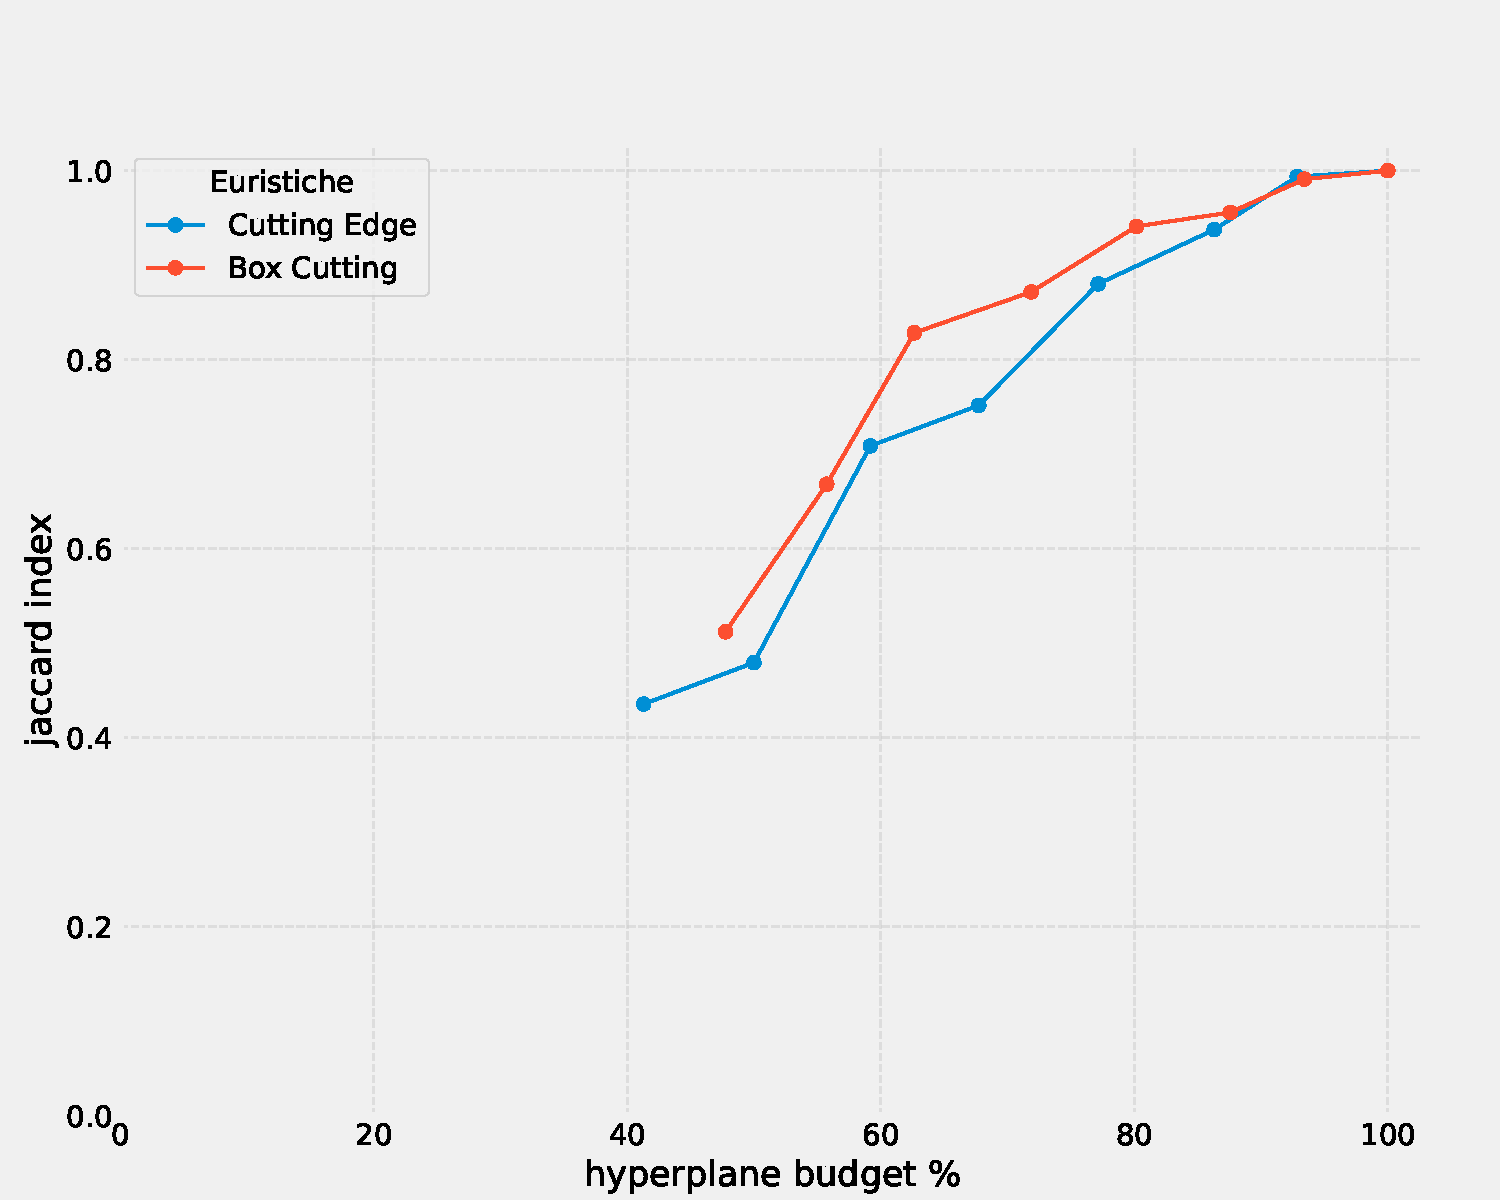
\includegraphics[width=0.7\textwidth]{media/report_ndim/ndim_jaccard.pdf} \\
        \caption{Andamento dell'accuratezza delle approssimazione degli algoritmi 
        al crescere del budget di iperpiani a disposizione}
\end{figure}

\begin{figure}[H]
    \centering
    \begin{minipage}[b]{0.45\textwidth}
        \centering
        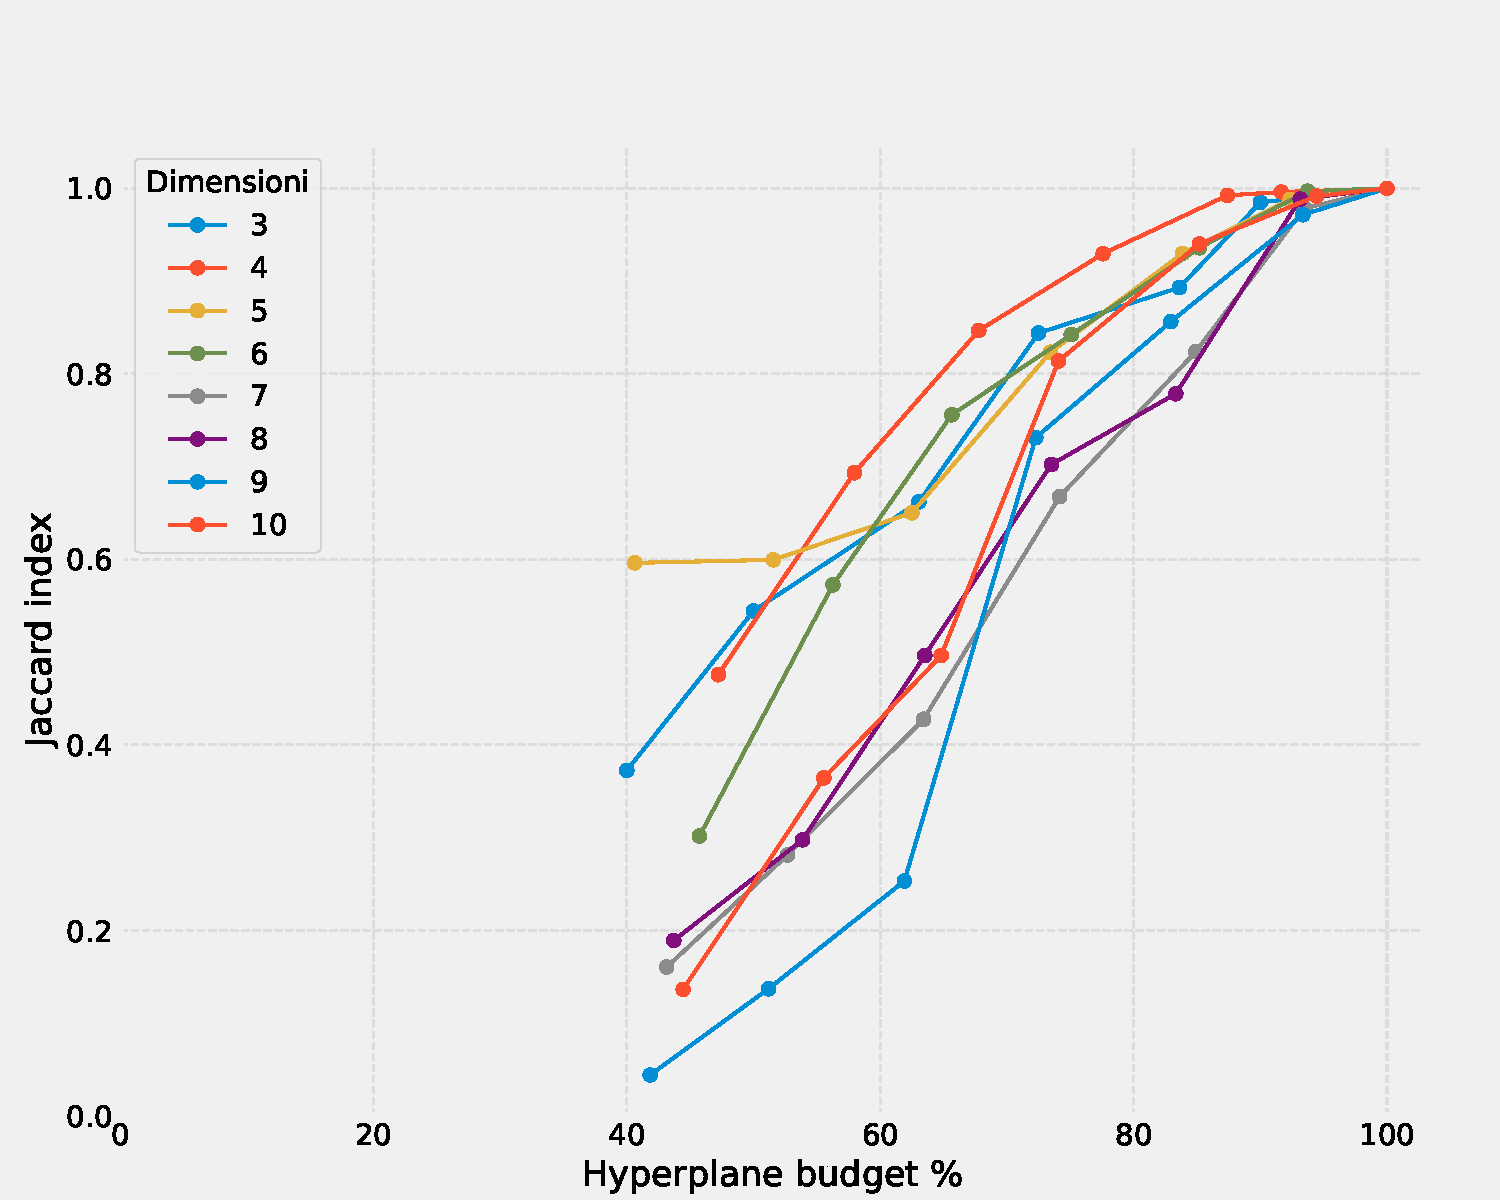
\includegraphics[width=\textwidth]{media/report_ndim/ndim_accuracy_diff_CE.pdf}
        \caption{Accuratezza dell'approssimazione di CuttingEdge al crescere di h.}
        \label{fig: acc_ce}
    \end{minipage}
    \hspace{0.05\textwidth}  % Spazio orizzontale tra le immagini
    \begin{minipage}[b]{0.45\textwidth}
        \centering
        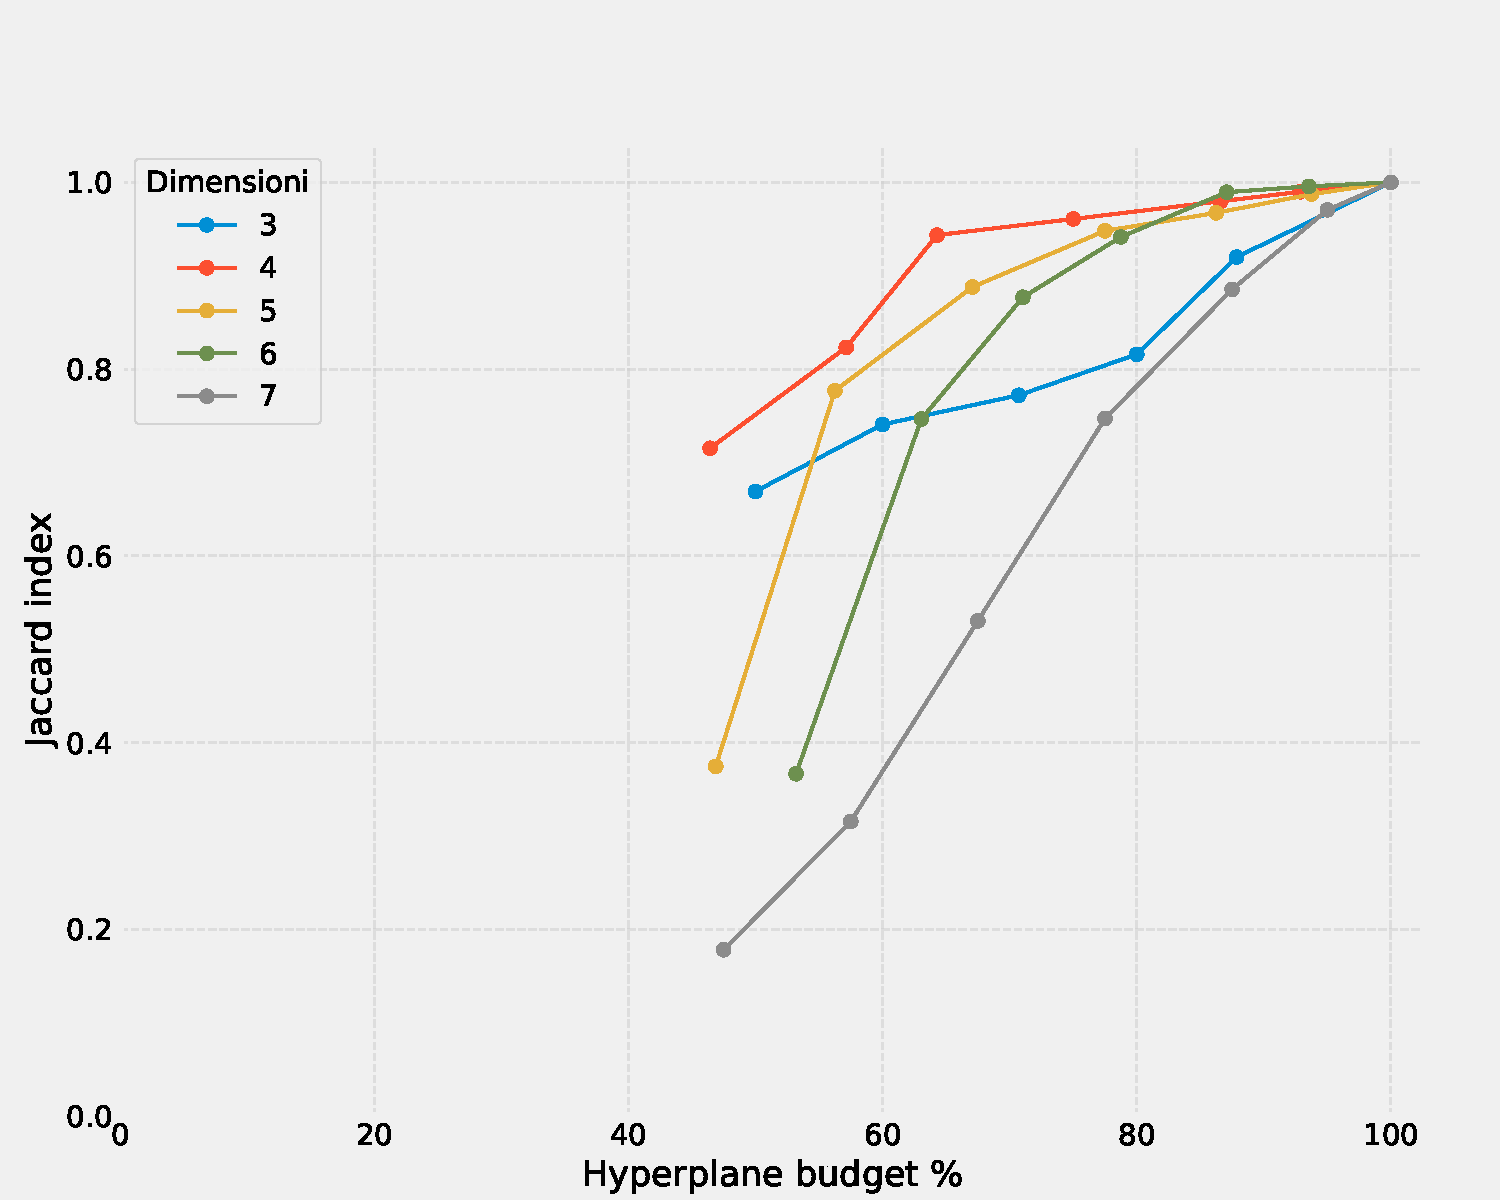
\includegraphics[width=\textwidth]{media/report_ndim/ndim_accuracy_diff_BC.pdf}
        \caption{Accuratezza dell'approssimazione di BoxCutting al crescere di h.}
        \label{fig: acc_bc}
    \end{minipage}
\end{figure}
Come previsto, il budget di iperpiani per l'approssimazione è incisivo sulla precisione
degli algoritmi. Nonostante ciò, è doveroso notare che entrambi gli algoritmi sembrano
avere un comportamento analogo al variare del budget di iperpiani.\\

Analizzando nello specifico il comportamento degli algritmi al variare delle dimensioni,
(Figure \ref*{fig: acc_ce} e \ref*{fig: acc_bc}) si nota un comportamento pressochè 
invariato per CuttingEdge mentre per BoxCutting il numero di dimensioni 
sembra marginalmente influenzare influenzarne l'accuratezza delle approssimazioni.

\begin{figure}[H]
    \centering
    \begin{tabular}{c}
        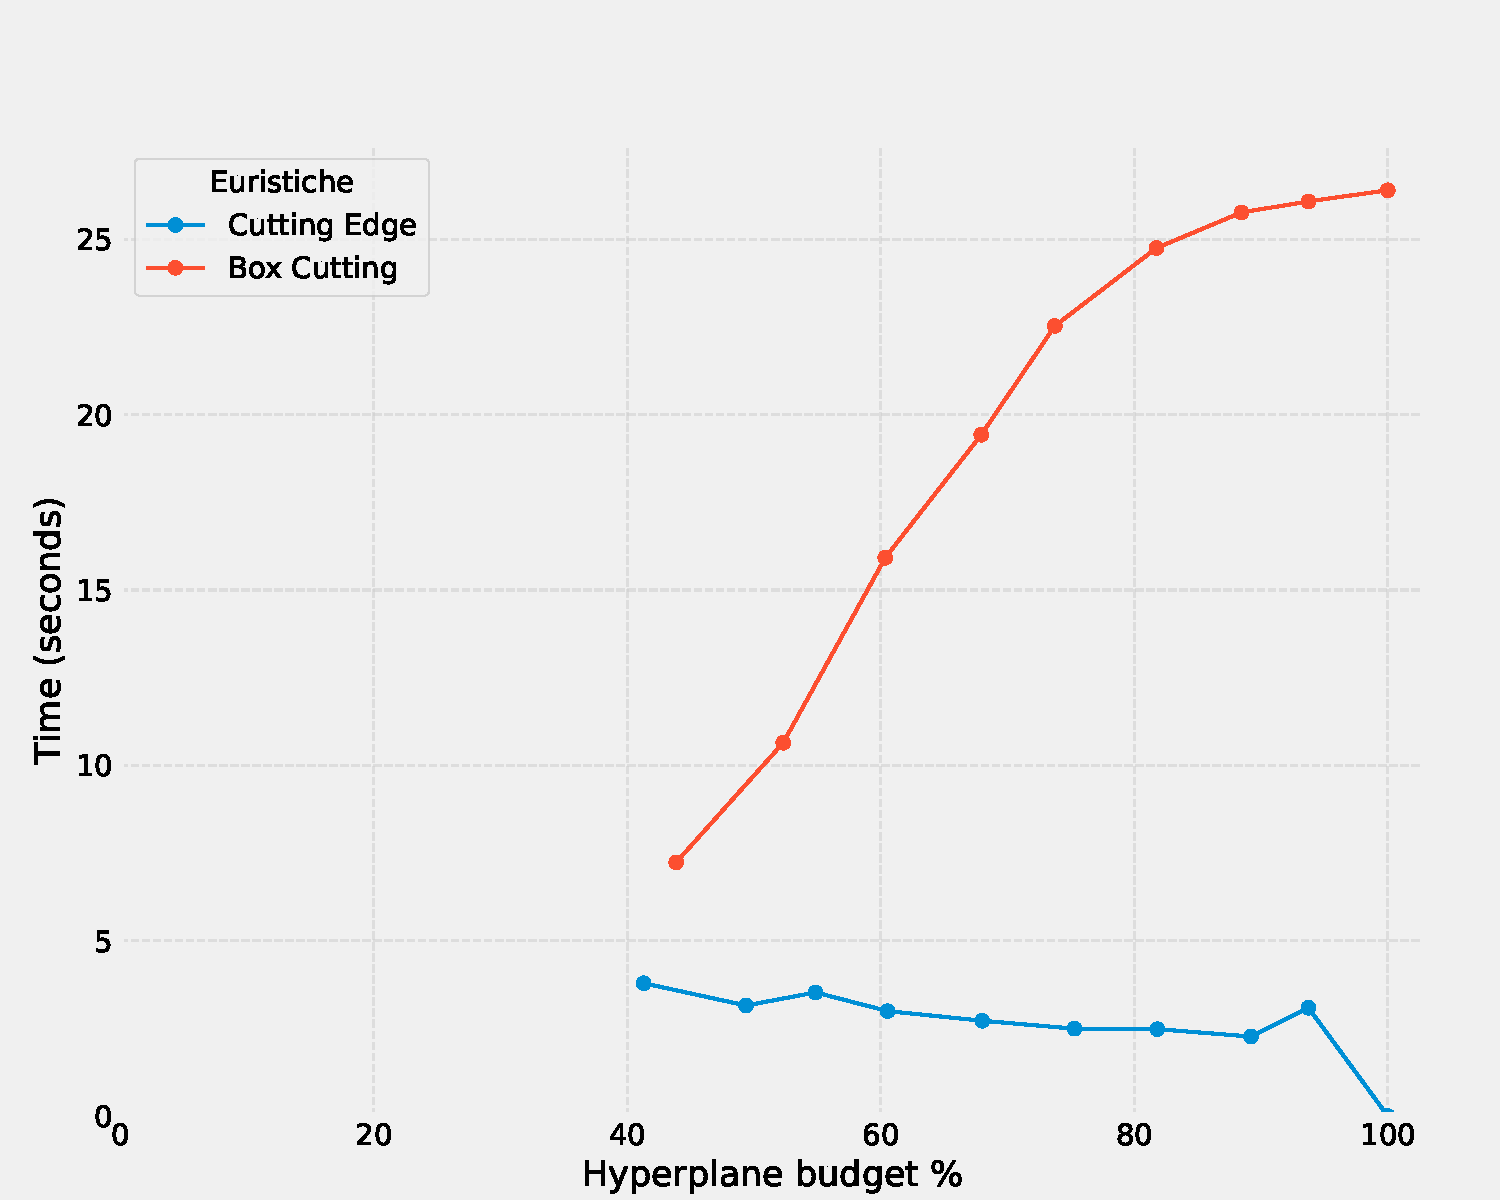
\includegraphics[width=0.7\textwidth]{media/report_ndim/ndim_time.pdf} \\
    \end{tabular}
    \caption{Grafico dei tempi di calcolo medi al variare del budget di iperpiani 
    a diposizione degli algoritmi scelti}
\end{figure}

Confrontando i tempi di calcolo si può notare una notevole differenza fra i due dovuta
principalmente dalla campacità di memorizzazione dei volumi calcolati per l'algoritmo 
CuttingEdge.


\begin{figure}[H] 
    \centering
    \begin{minipage}[b]{0.45\textwidth}
        \centering
        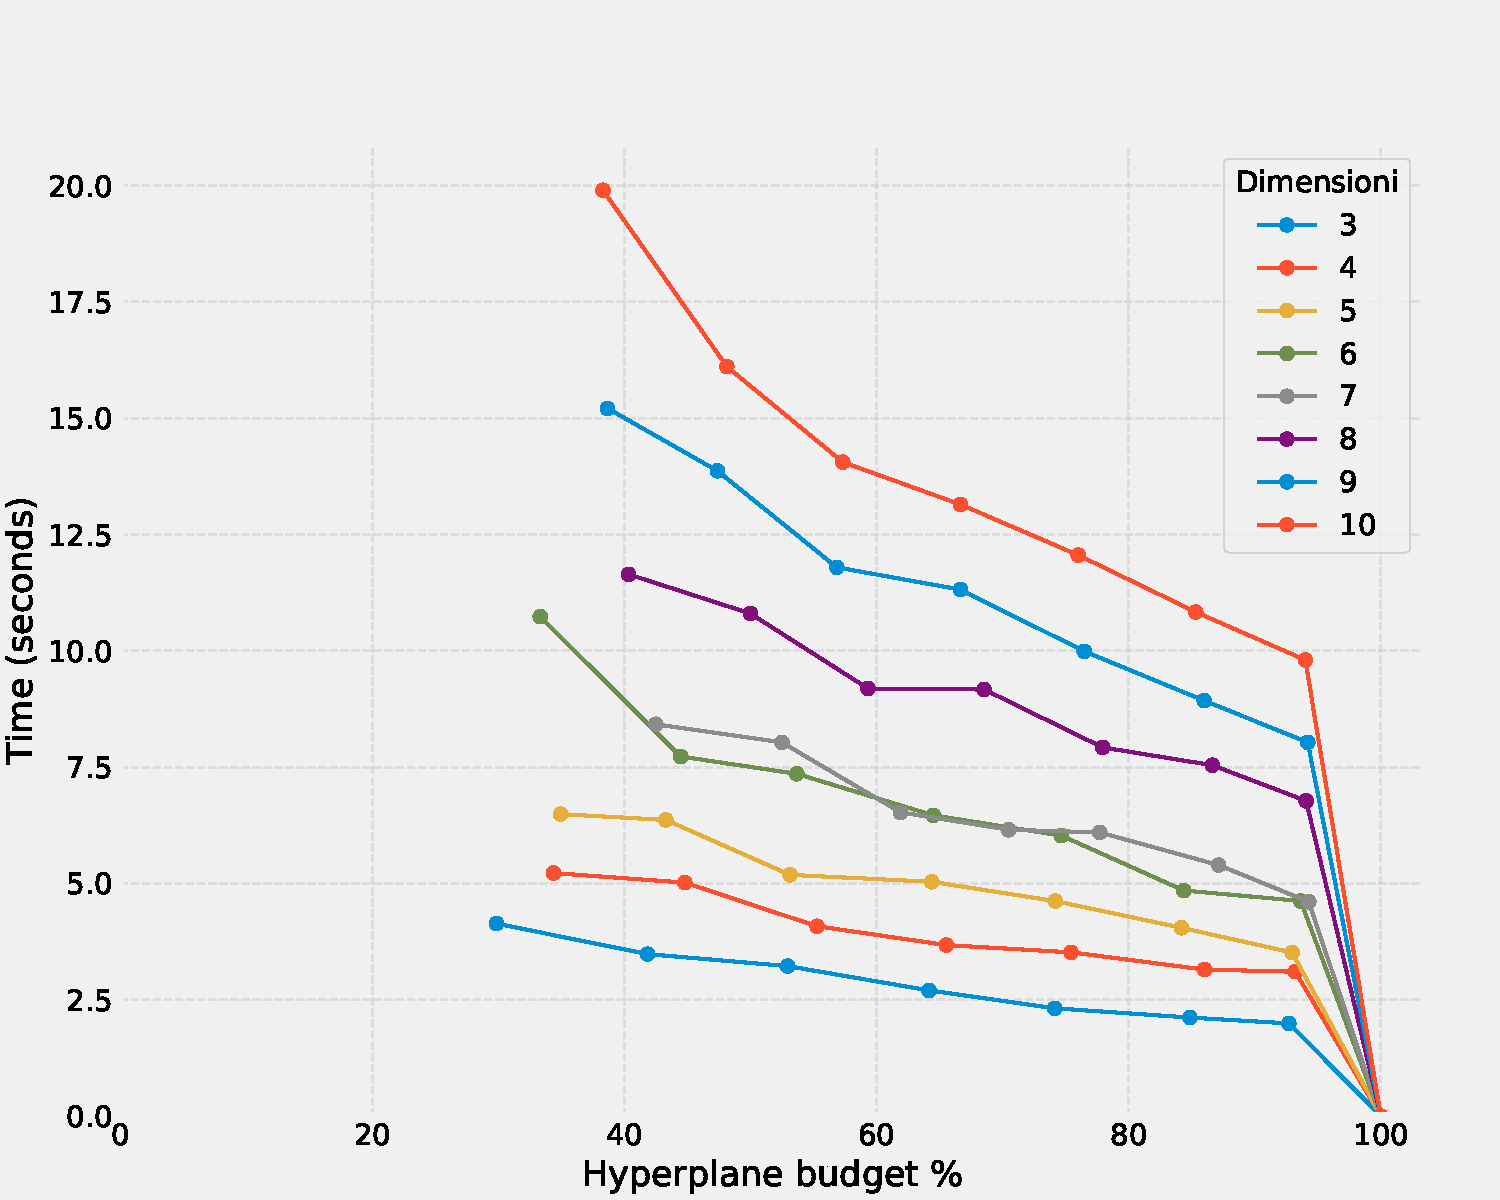
\includegraphics[width=\textwidth]{media/report_ndim/ndim_time_diff_CE.pdf}
        \caption{Tempi di esecuzione dell'euristica CuttingEdge al variare del 
        budget di iperpiani.}
        \label{fig: disp_ce}
    \end{minipage}
    \hspace{0.05\textwidth}  % Spazio orizzontale tra le immagini
    \begin{minipage}[b]{0.45\textwidth}
        \centering
        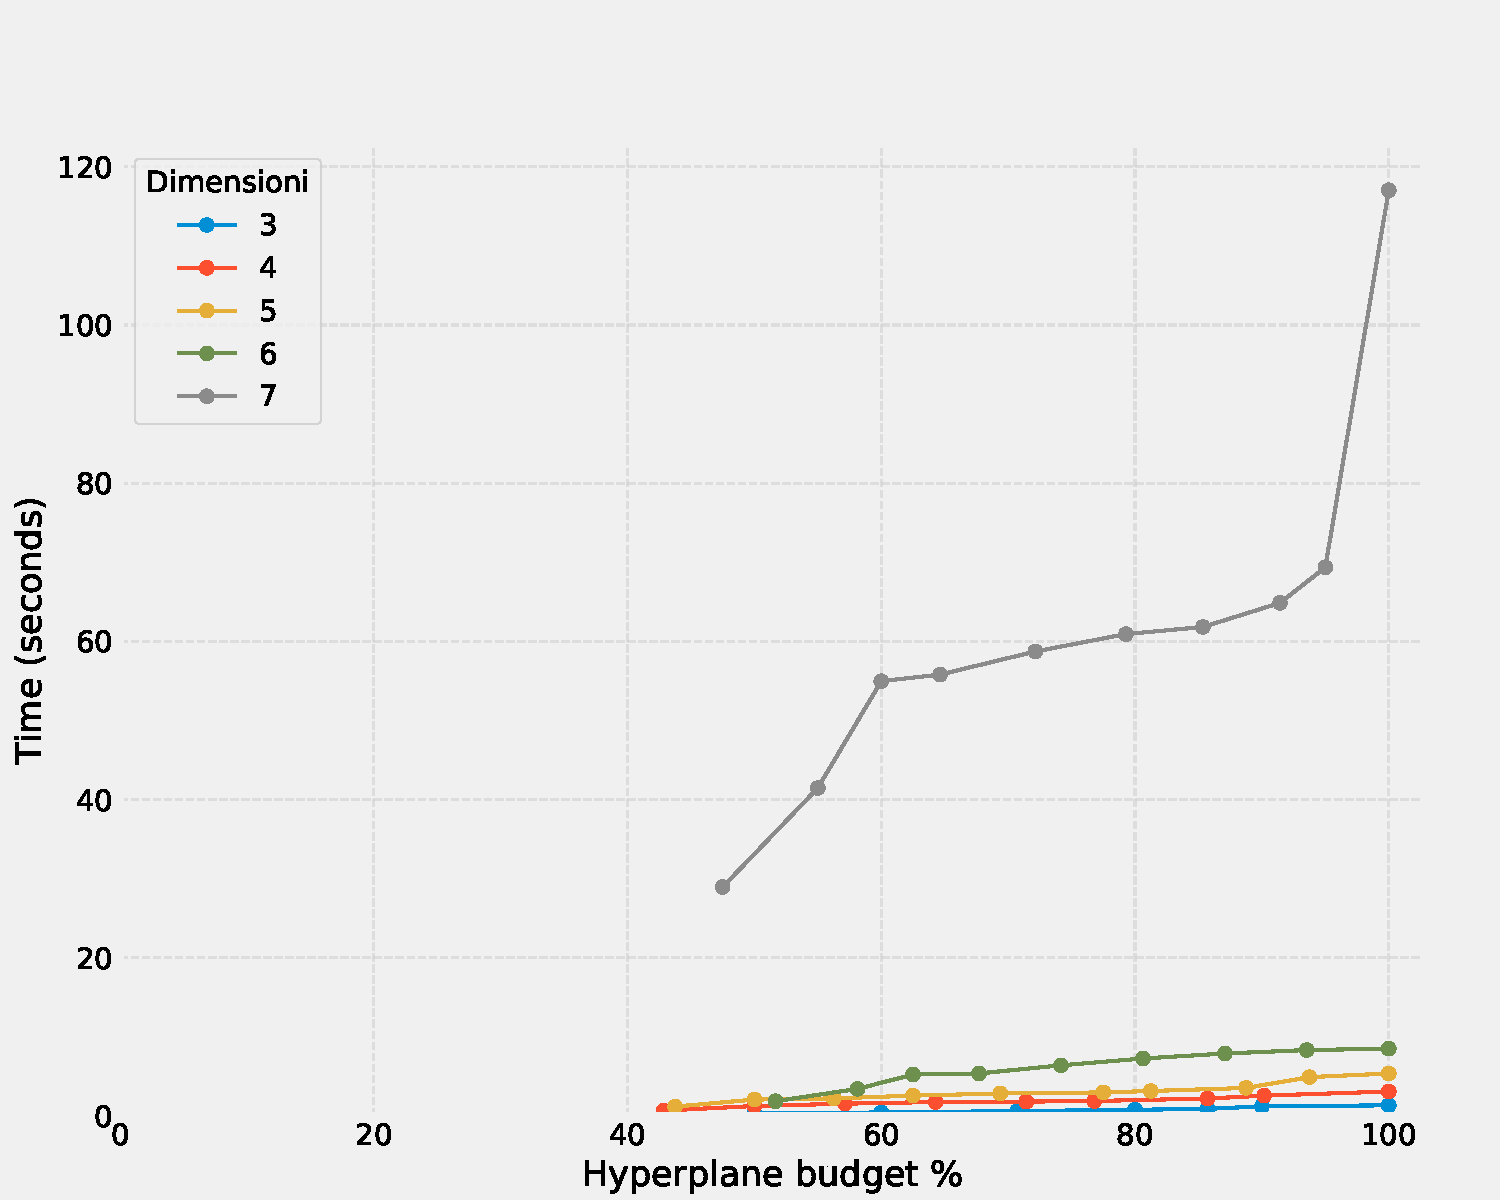
\includegraphics[width=\textwidth]{media/report_ndim/ndim_time_diff_BC.pdf}
        \caption{Tempi di esecuzione dell'euristica BoxCutting al variare 
        del budget di iperpiani.}
        \label{fig: disp_bc}
    \end{minipage}
\end{figure}

\begin{figure}[H]
    \centering
    \begin{minipage}[b]{0.45\textwidth}
        \centering
        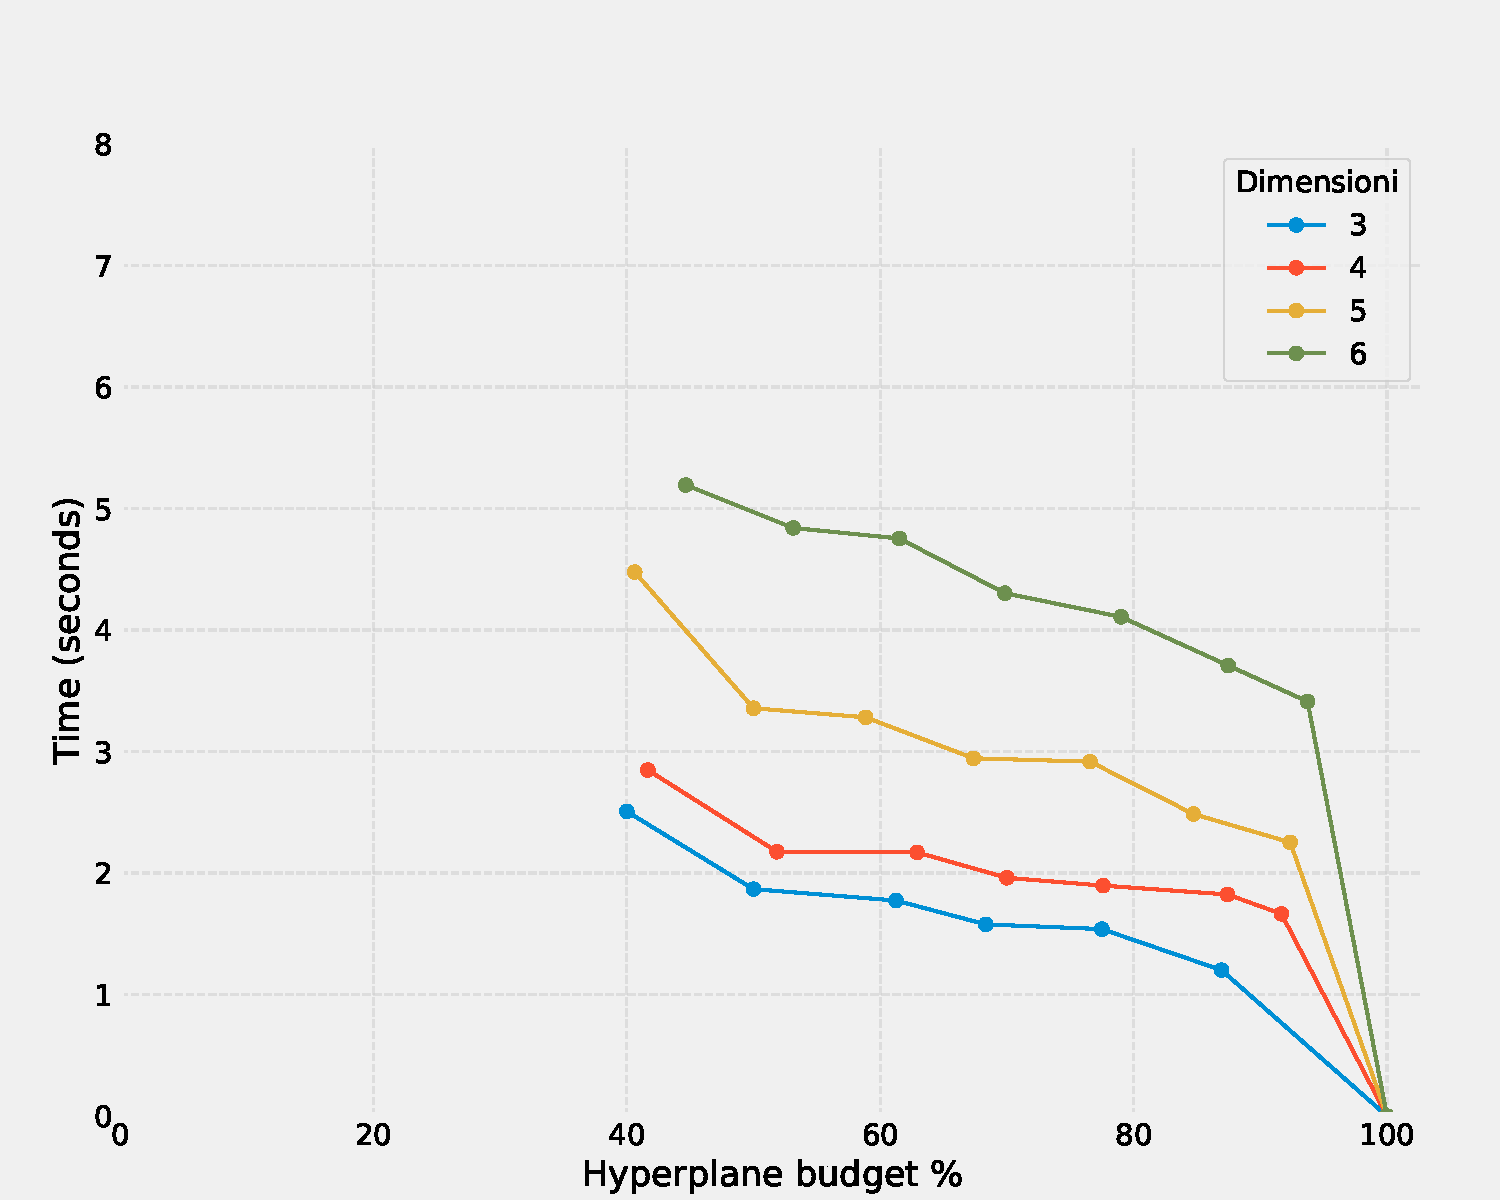
\includegraphics[width=\textwidth]{media/report_ndim/ndim_time_diff_CE_under7.pdf}
        \caption{Tempi di esecuzione dell'euristica CuttingEdge al variare 
        del budget di iperpiani per le dimensioni comprese tra 3 e 6, 
        filtrando le dimensioni superiori per una migliore visualizzazione.}
        \label{fig: disp_ce_sub7}
    \end{minipage}
    \hspace{0.05\textwidth}  % Spazio orizzontale tra le immagini
    \begin{minipage}[b]{0.45\textwidth}
        \centering
        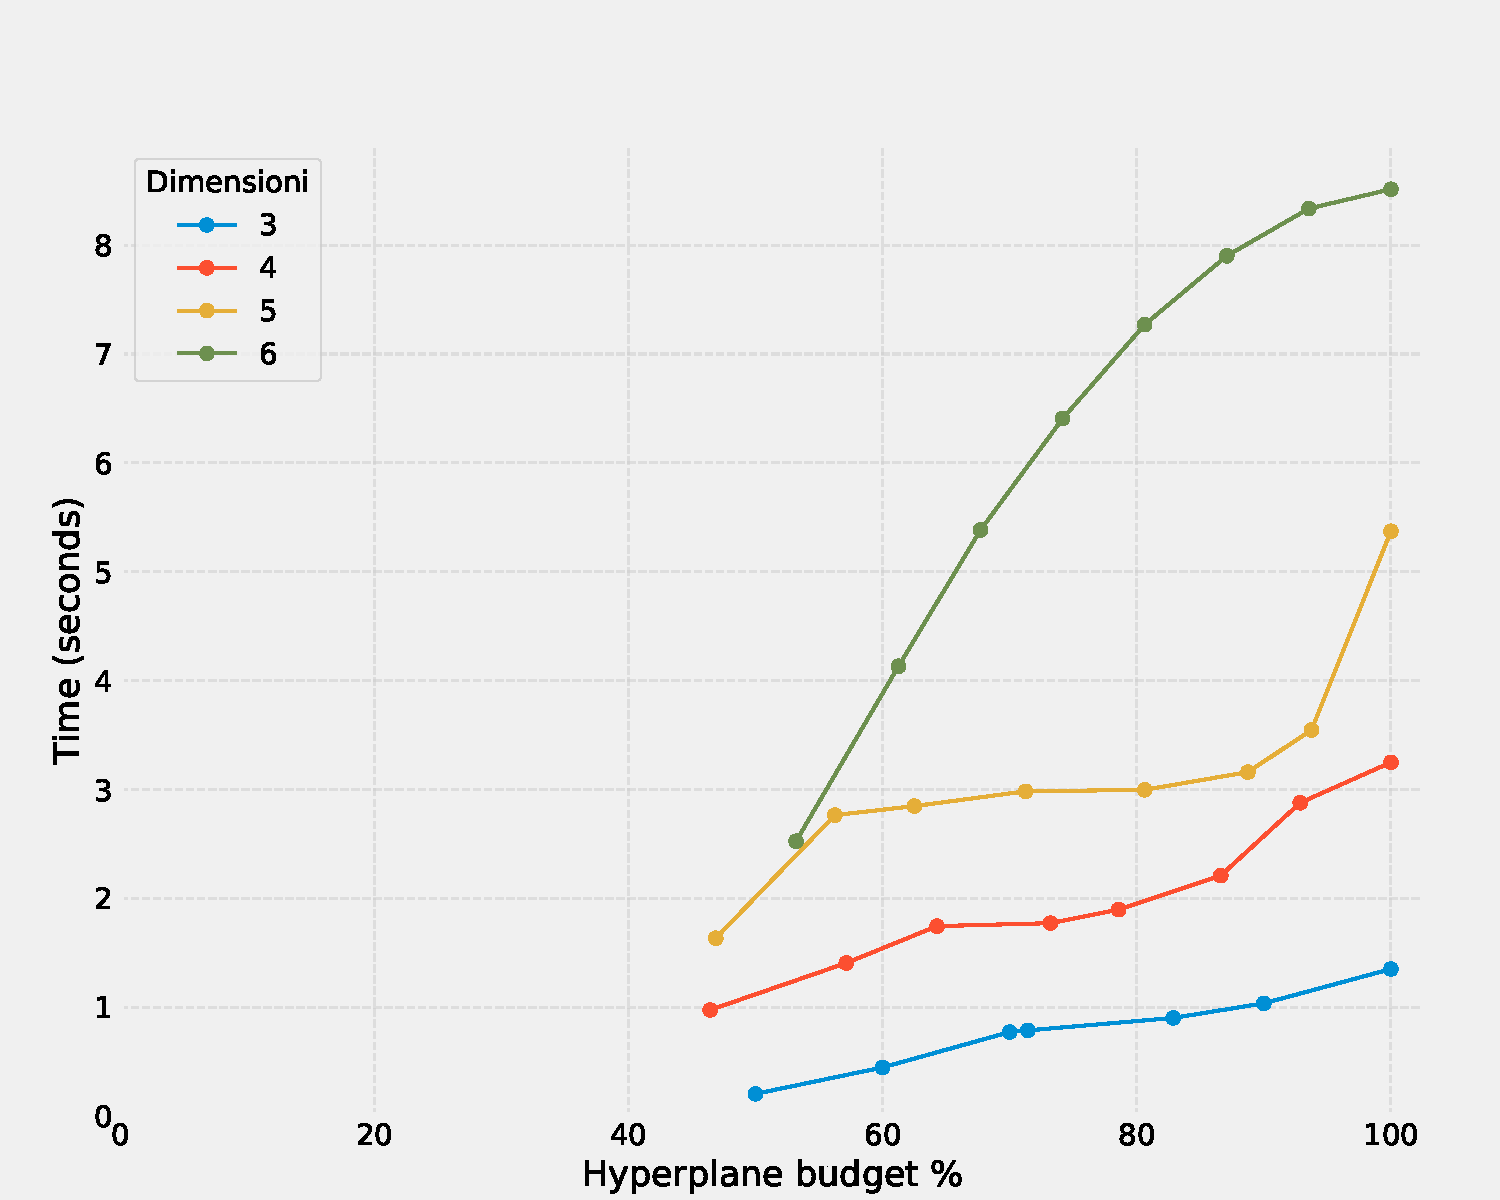
\includegraphics[width=\textwidth]{media/report_ndim/ndim_time_diff_BC_under7.pdf}
        \caption{Tempi di esecuzione dell'euristica BoxCutting per lo stesso 
        intervallo di dimensioni.\\
        \\}
        \label{fig: disp_bc_sub7}
    \end{minipage}
\end{figure}

Come si può evincere dai grafici nelle Figure \ref{fig: disp_ce} \ref{fig: disp_bc},
al crescere delle dimensioni dei politopi di partenza l'euristica BoxCutting 
subisce una notevole crescità del tempo computazionale, mentre CuttingEdge 
riesce a mantenere una crescita costante e predicibile.

Confrontando le dimensioni per le quali i due algoritmi risultano comparabili, 
ovvero dalla 3 alla 6 (Figure \ref{fig: disp_ce_sub7} \ref{fig: disp_bc_sub7}), 
si può osservare che entrambi gli algoritmi 
presentano tempi di esecuzione simili, ma con andamenti di crescita opposti. 
In particolare, l'algoritmo CuttingEdge mostra un tempo di esecuzione decrescente 
all'aumentare del budget di iperpiani, mentre l'algoritmo BoxCutting evidenzia 
una crescita dei tempi con l'incremento del budget di iperpiani. 
Questa caratteristica può renderli adatti per scopi differenti.\\

